\documentclass[a4paper, 11pt]{article}
\setlength{\topmargin}{0in}
\setlength{\textheight}{8in}
\setlength{\oddsidemargin}{.1in}
\setlength{\textwidth}{6in}

\usepackage{multirow}
\usepackage{float}
\usepackage{array}
\usepackage[document]{ragged2e}
\usepackage{comment} 
\usepackage{subcaption}
\usepackage{amssymb,amsmath}

\usepackage{datetime}

\newdateformat{mydate}{\monthname[\THEMONTH] \THEYEAR}

\newcolumntype{L}{>{\centering\arraybackslash}m{3cm}}

\usepackage{graphicx}
\graphicspath{{images/}}

\begin{document}


\LARGE\title{User Modelling in Search for People with Autism}

\LARGE\author{Author: \textbf{Esha Massand}, Supervisor: \textbf{Keith Mannock}\\
\\
MSc Computer Science\\Department of Computer Science and Information Systems\\Birkbeck College, University of London\\\\\\Project report submitted in partial fulfilment of the requirement for the \\MSc in Computer Science\date{\mydate\today}
\\\
}

\normalsize


\maketitle


\section*{Abstract}
\begin{justify}
This project report presents my research and the development of a prototype web application to assist users with Autism when they search the web. The system has modelled user interactions with the search process into a user profile for this category of users, integrating insights from the core features of autism into the model. The system is integrated with an infra-red, motion controlled, user interface component to assist users with Autism during search. The project provides insights into how search can be improved for users with Autism.\\
\end{justify}
\begin{verbatim}






\end{verbatim}

\begin{justify}
This project is substantially the result of my own work, expressed in my own words, except where explicitly indicated in the text. I give my permission for it to be submitted to a Plagiarism Detection Service. This proposal may be freely copied and distributed provided the source is explicitly acknowledged.
\end{justify}



\begin{center}
word count (project text only) :
\end{center}

\clearpage
\tableofcontents
\clearpage

\section*{Abbreviations}
\begin{tabular}{l l }
API & Application Programming Interface\\
AQ & Autism Quotient\\
ASD & Autism Spectrum Disorder\\
DSM & Diagnostic and Statistical Manual\\
GCS & Google Custom Search\\
HCI & Human Computer Interaction\\
HTTP & Hypertext Transfer Protocol\\
JSON & JavaScript Object Notation\\
IDE & Integrated Development Environment\\
KWIC & Key Word In Context\\
LEAP & LEAP Motion Controller\\
REST & Representational state transfer\\
RIFT & Oculus Rift Virtual Reality Head Mounted Display\\
TDD & Test Driven Development\\
UI & User Interface\\
UX & User Experience\\
VR & Virtual Reality\\
\end{tabular}

\section*{Definitions}

\begin{tabular}{l p{11cm}  }
Autism & Autism is amongst the most common neuro-developmental condition and it is currently estimated that 1/68 children meet criteria for Autism Spectrum \cite{CDC}. Autism is five times more common amongst boys than girls (1/42 boys, and 1/189 girls). According to the Diagnostic and Statistical Manual (2013), Autism is characterised by persistent and early deficits in reciprocal social interaction and repetitive behaviours. Individuals vary from high functioning to low functioning (along a spectrum), with behaviours emerging around 2 to 3 years of age.\\


Stereotyped User Model & Stereotyped user models infer characteristics about a user from data gathered from other users within that distinct subset. They can be built quickly using clusters of characteristics of groups of individuals. 

\end{tabular}
\clearpage

\section*{Search Engine Measures}
\newcommand{\cfplus}{\mathbin{\genfrac{}{}{0pt}{}{}{+}}}

\subsection*{Precision}
The field of information retrieval defines precision as the fraction of retrieved documents that are relevant to the query. 

\begin{equation*}
Precision
=\frac{|(relevant\ documents) \land (retrieved\ documents)|}{|(retrieved\ documents)|}
\end{equation*}

\subsection*{Recall}
The field of information retrieval defines recall as the fraction of relevant documents that are retrieved by the search query. 

\begin{equation*}
Recall
=\frac{|(relevant\ documents) \land (retrieved\ documents)|}{|(relevant\ documents)|}
\end{equation*}
\clearpage

\section{Introduction}\label{intro}

\begin{comment}
Contains a brief outline of the topic as a whole
Then state the aim and objectives of the project
What was the purpose of the project and what did it set out to investigate?
At the end of the introduction, provide a road map for the
remainder of the report
\end{comment}

This project report presents the development and evaluation of a prototype web-browser based application to assist users with Autism when they search the web. The application is hereafter referred to as Jellibeans \footnote{Jellibeans are a rainbow of colours, different sizes and shades, and the name represents the difference in style of processing of individuals with ASD.}. Jellibeans utilises gesture and hand movement data recorded using the Leap Motion Controller (LEAP). 
\vspace{5mm}

In programmatic terms, Jellibeans is designed to implement a research-guided user model in search. The development of this user model consisted of iterations of the `research, development, test, evaluate' lifecycle. I conducted research to identify the preferences within search, and the differences in user queries formed by individuals with Autism, by conducting surveys and collecting and analysing search behaviour patterns from people with and without Autism. Using these data I built a set of features into search, to guide the user through forming a more complete search query. Development and evaluation included the implementation and testing of the features, and further implementation and revision of the software to enhance the search process and the precision of the search engine for the users' intended search query. 
\vspace{5mm}

Jellibeans integrates a motion controlled user interface (UI) using the LEAP motion controller. The interface is very dynamic as opposed to static, and can hold users' attention for longer periods of time. In the past, users with Autism have struggled to maintain their attention to sift through the large number of search results. In line with the attention difficulties individuals with Autism face, Jellibeans has been designed to reduce the amount of text on the search results page, presenting only 3 results per page, instead of the default 10. 

\vspace{5mm}
Despite Autism being amongst the most common neuro-developmental condition (1/68 children meet criteria for Autism Spectrum \cite{CDC}), no user model has yet been developed for Autism within Search. In the current project, I describe my efforts to build a user model within search for individuals with Autism.

\begin{comment}
Individual characteristics of each user will be measured using a 50 item questionnaire, the Autism Quotient (AQ \cite{Baron Cohen et al}) which measures tendency towards autistic traits. A score of 32 or higher indicates a strong likelihood of Autism or Aspergers syndrome (the questionnaire has a 79\% sensitivity score). Individuals who score highly on the AQ will be offered the current user model for their search. The questionnaire data will be stored in the user's Google+ profile????
\subsection {User Models in Search}
\subsection {Rule and Transformation Engine}
\subsection {Motion Controlled Navigation in Search}


Are there any specific work packages that need to be done? If so, list those out here.
\end{comment}

\subsection {Background Research}\label{background} 

\begin{comment}
What is the problem we are trying to solve?
define concepts and previous approaches.
This chapter should focus on the context that you are operating in, e.g., by describing typical applications
alternative tools and development approaches and how they have been used in practice
alternative systems and what they achieve and do not achieve
This should be a synopsis of the relevant part of your project proposal (do not just copy your proposal)
Restrict yourself to what'€™s relevant to the specific context of your project (the proposal can have a more general look at the
state-of-the-art)
\end{comment}

According to the Diagnostic and Statistical Manual \cite{CDC}, Autism is characterised by persistent and early deficits in reciprocal social interaction, so interaction with computers is prominent in this group. It is also well established that individuals with Autism are more engaged when using technology that is receptive and interactive (e.g., games, responsive consoles, motion controlled devices) compared to technology that is not \cite{motioncontrollerforautism}. This project will combine interactive, motion recognition hardware with search to also improve the UI (user interface) of search for individuals with Autism.\\

\vspace{5mm}
Research has shown that people with Autism are less context-sensitive and prefer a more detail-focused processing style \cite{mottron}. There is good reason to postulate then, that web-search queries are formed very differently to the typical population. Generally speaking, individuals with Autism prefer, and are more likely to engage in an item-specific, or detailed processing style, resulting in web-search queries that are more likely formed of single-order associations. In addition to a detailed, item-specific processing style, individuals with Autism are also less likely to engage in a contextual processing style. For example in a search for `Guitar', a contextual style of processing would imply an awareness that the word is related to `Piano', but also that both words are hierarchically related to `Instrument'. In day to day life, a major factor determining the effectiveness of working-memory (the transient holding and processing of information for updating, learning and comprehension), and the amount and quality of information that an individual can recall and enter into the web-search, is greatly influenced by the number of cues that are available at the time. For example, if presented with a list of 50 items to remember, you are more likely to remember that I presented `Zebra' if I tell you that I presented an animal. This type of `cued' recall can be used to bolster recall of information for people with Autism, and is a technique that will be applied in the current project. \\

\subsection{The Problems with Current Web-Search}\label{What should search offer people with Autism}

The Internet is one of the largest resources of information. Search engines allow users to collate hundreds of links on a single topic, using only a few words or phrases. The typical user sorts the returned results into `relevant' or `irrelevant' categories, flexibly shifting (mentally) between one result and the next, to determine the relevance of each page returned by the search engine. Search allows the user to assimilate the information on the page into their knowledge and is an important learning tool. For people with Autism, the requirement is no different, however, current search is not adequate. A large body of research has shown that `mental shifts' are a known area of weakness for people with Autism \cite{disengagement}. The information is therefore harder to assimilate or learn, and judging the relevance of each document becomes near impossible. One successful therapeutic technique to increase the assimilation of information for individuals with Autism is to present it in clearer, smaller amounts \cite{AdultsWithAutism}. This technique avoids overwhelming individuals, and although less information is presented as a whole, whatever is presented to the user becomes `digestible' and ultimately, the information as a whole becomes more understandable.  \\
\vspace{5mm}
One of the first aims of the current project was to build a synthesis of three leading search engines, to ensure the best possible results were retrieved by Jellibeans and presented to the user. The first stage was to therefore build the combination search engine and test the results on a user group with Autism. The goal of the research was to understand if the synthesis of the search engines enhanced search experience (in other words were users happy with the combination search), or, whether the results introduced redundancies or oddities in the results (some users may not use a certain search engine because they do not find the results helpful).\\
\vspace{5mm}

Search queries usually fall into one of three broad categories.  `Do' queries which characterise transactions between the user and the search engine, for example when the user wants to do something such as \textit{buy a plane ticket}, \textit{listen to a song} or, \textit{download a screensaver}. `Know' type queries, which are informational in nature, usually covering a broad topic, for example, the \textit{name of a band} or \textit{restaurant in London}, \textit{trucks}, or \textit{Colorado}. The third broad category is `Go' type queries, which are navigational in nature, for example, searching for a particular home page on the web, \textit{YouTube} or \textit{American Airlines}. There are also many stages to the search process \cite{seo}. After identifying the information need, the user must formulate a search query. The user must browse through results once the query has been entered into a search engine. The whole process can be repeated if the user is not satisfied. 

\begin{enumerate}
\item{Experience the need for an answer,
solution, or piece of information.}
\item{Formulate that need in a string of words and phrases, also known as “the query.”}
\item{Enter the query into a search engine.}
\item{Browse through the results for a match.}
\item{Click on a result}
\item{Scan for a solution, or a link to that solution.}
\item{If unsatisfied, return to the search results and browse for another link or ...}
\item{Perform a new search with refinements to the query}
\label{search flows}
\end {enumerate}


\subsection{Design Patterns for Web Applications}

Search engines like Google apply strong reduction techniques to navigation of the web. For example, one common way this reduction pattern is implemented is by assuming the behaviour of the current user is similar to the behaviour of other users in similar situations. This is often seen in recommendation engines, e.g., Amazon. The principle applied by Google is to `make it easy' for the user \cite{googleTerms}, by assuming that users form search queries similarly, and returning similar results to those users.

\vspace{5mm}
As we have seen in the introduction, users with Autism behave in different ways to typical users when navigating search. Users with Autism do not use the same key phrases when looking for documents with several attributes, i.e., queries that would be best formulated using several iterations of search, or multiple search parameters. This leads to an ineffective search; one that requires users to sift through results which are in large-part irrelevant, and a bad user experience.  
\vspace{5mm}
Parametric search queries allow users to define parameters in an increasingly logical and structured way. As an example, consider the experience of searching for flights to a particular holiday destination, or for a person. This requires high cognitive `load' (remembering and manipulating arrival, departure, destination, timings, airlines, seat preferences etc.) so searches are often structured using fixed options (see Figure~\ref{exped}).

\begin{figure}[H]
\begin{center}
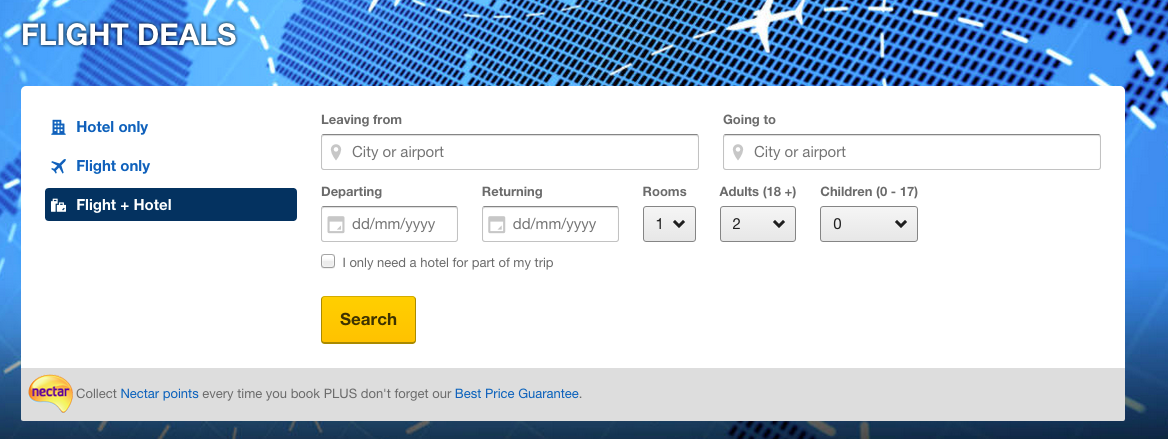
\includegraphics[scale=0.3]{expedia}\\

\caption{Expedia Parametric Search Example}
\label{exped}
\end{center}
\end{figure}

For typical users, parametric search is more structured, and in some circumstances seems more natural than a free – keyword search. It makes search queries easier to formulate in situations where there is a high cognitive load.  We can apply this idea to web search for people with Autism, by asking them to enter criteria that can be applied to subgroups of search queries. Parametric search can assist the user with capturing the search parameters that are useful for a query it does not ultimately reduce the number of search results returned; the possibility of a large result set is most definitely true. However, when used in addition to the original search query itself, the parametric search will refine the user'€™s search results in line with their search query, ultimately leading to a higher precision for the search engine.
\vspace{5mm}
One of the aims of the study is to reduce the amount of textual information on the webpage presented to the user, so the solution implemented here tries to find a balance between these two aims.\\  


\subsection{Motion controllers}
Individuals with Autism have poor attention \cite{attention}. The static 2-dimensional interface of many current search engines is unlikely to maintain adequate (sustained) interest levels. Individuals (and especially teenagers) with Autism spend a substantial amount of their time using computers, web, portable or console devices \cite{Shane and Albert}, as they find these more stimulating and attention-grabbing. For these individuals, computer-based technologies provide a stable, consistent learning environment that can be customized \cite{moore}. Furthermore, motion recognition devices can be programmed to make consistent responses to environmental triggers. These controlled and interactive environments have shown promise for improving social communication skills and reducing repetitive behaviours \cite{gameshealth}. For the current project a motion-controlled learning environment will be bolstered to improve attention within search for people with autism. 

\begin{figure}[H]
\begin{center}
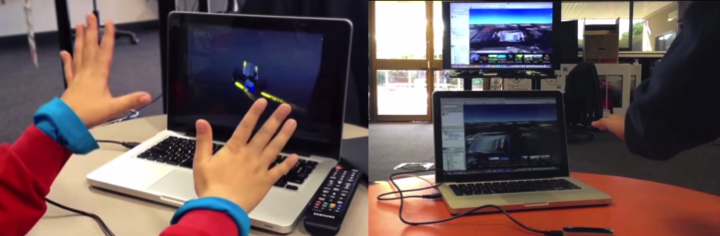
\includegraphics[scale=0.5]{vision}\\
\caption{Envisioned UI component for the project \cite{leap}.}
\label{vision}
\end{center}
\end{figure}


\subsection{Summary}

As search can be compartmentalised into `Do', `Know' and `Go' type queries, it provides a natural way to tackle the issue of simplifying the search process for people with Autism. Users first identify the type of search they would like to carry out, the search engine can better phrase a question to guide the user through their informational demand. Each stage of the search process described above, can be better tailored towards providing a concrete and unambiguous experience for the user with Autism, and reducing the amount of text on the page. When using Jellibeans query formulation, the user will be assisted through the process of formulating a search query (much like a parametric search engine form for example when you buy a car, you fill out many criteria which must be simultaneously searched for). Concretely phrased questions will be aided by suggestions that appear laterally on the page. These suggestions can be added into the search query without the need to type them in, just by using natural hand movements, tracked by the LEAP motion controller. The suggestions also serve as cues for the user, and to simplify the search process for them.  The UI component will make the whole experience more interactive and the search engine more receptive to user input. The process of forming an search query thus becomes more tightly defined compared to the current systems for web search, the process will be more predictable, and the size of the result-set will be adapted towards users with Autism.  

\subsection {Aims for Jellibeans}
The goal of the project is to build a prototype search tool that assists users with Autism search and navigate the web. These prototype features will be tested on a group of users with Autism. The final product will be integrated within a motion-controlled environment. The prototype will be modified accordingly in line with the outcome of several stages of user research.\\ The core features of Jellibeans are:

\begin{enumerate}
\item  {To implement and test a combination search web application that synthesises the results from three of the largest and most popular engines; Google, Bing and Yahoo \cite{adam}.}

\item {The design and implementation of a user model of Autism to filter user search results. This will be a \textit{stereotyped} model, i.e., some characteristics of the model will be based upon the user's demographic data, other characteristics will be inferred from the Autism subset of users (see Section~\ref{usermodel} for an explanation of the different types of user models.)}

\item {Key Word In Context search; returning query terms in context, within small snippets (not verbally-overloaded).}

\item {Prioritisation of results which have first-order semantic relations to the query words i.e., they appear in matched context to the search query.}

\item {Motion controlled UI (see Figure~\ref{vision}).}
\end{enumerate}





\section{Project Trailer}

\begin{figure}[H]
\begin{center}
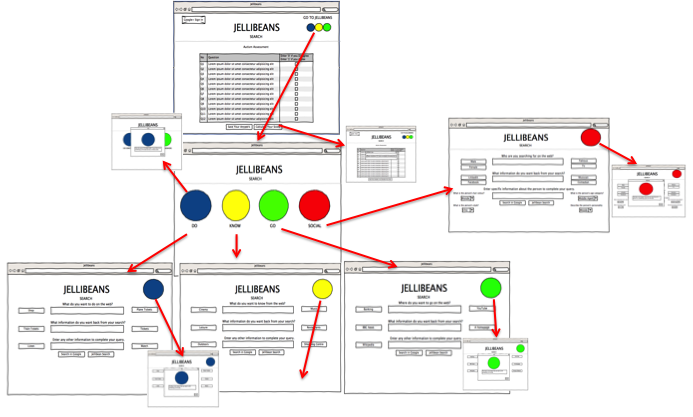
\includegraphics[scale=0.7]{JellibeanUserFlow.png}
\end{center}
\caption{Wireframe Sketches for Jellibeans User Flow}
\label{JBeanUserFlow}
\end{figure}

\subsection{Description of What Jellibeans Does}
\begin{enumerate}
\item{Jellibeans is a web-browser based application to assist users with Autism when they search the web. Jellibeans can be found at http://esha.mseth.co. }
\item{Jellibeans utilises a \textit{stereotyped} user model of Autism for Web Search. The features of the model were determined following analyses of survey responses gathered from individuals with Autism or a high occurrence of autism-like symptoms. The survey was administered online using a web-based survey engine \cite{surveymonkey}, and focused on identifying the differences in user search query generation for people with autism (see Figure~\ref{JBeanUserFlow}).}
\item{Following the insights gathered from the first set of research findings above, Jellibeans employed a parametric-like search, and include suggestions to guide the user towards forming succinct and accurate search queries.}
\item{Jellibeans was integrated with Google+, to allow the user to sign in and have their profile picture and name displayed, enhancing the feel of a personalised search engine.}
\item{Jellibeans allows users to get feedback on the level of their autism-like symptoms. The Autism Quotient \cite{Baron Cohen et al}, a scientifically validated screening tool for autism spectrum disorders will feature on the Jellibean homepage, and users can retrieve their score and save their responses for each question to a local file for their reference (the file is formatted for Microsoft Excel).}
\item{Jellibeans prioritises and displays the three highest precision search results for users. The goal of Jellibeans is to increase precision of the search results that are returned. Recall of the engine is sacrificed in line with the demands of the user model, to have less textual information on the page.}
\item{Jellibeans reduces the amount of text on the webpage by having results display on a modal (a hovering display panel on the page) which can be easily closed, and reopened to display results (see Figure~\ref{resultsModal}).

\begin{figure}[H]
\begin{center}
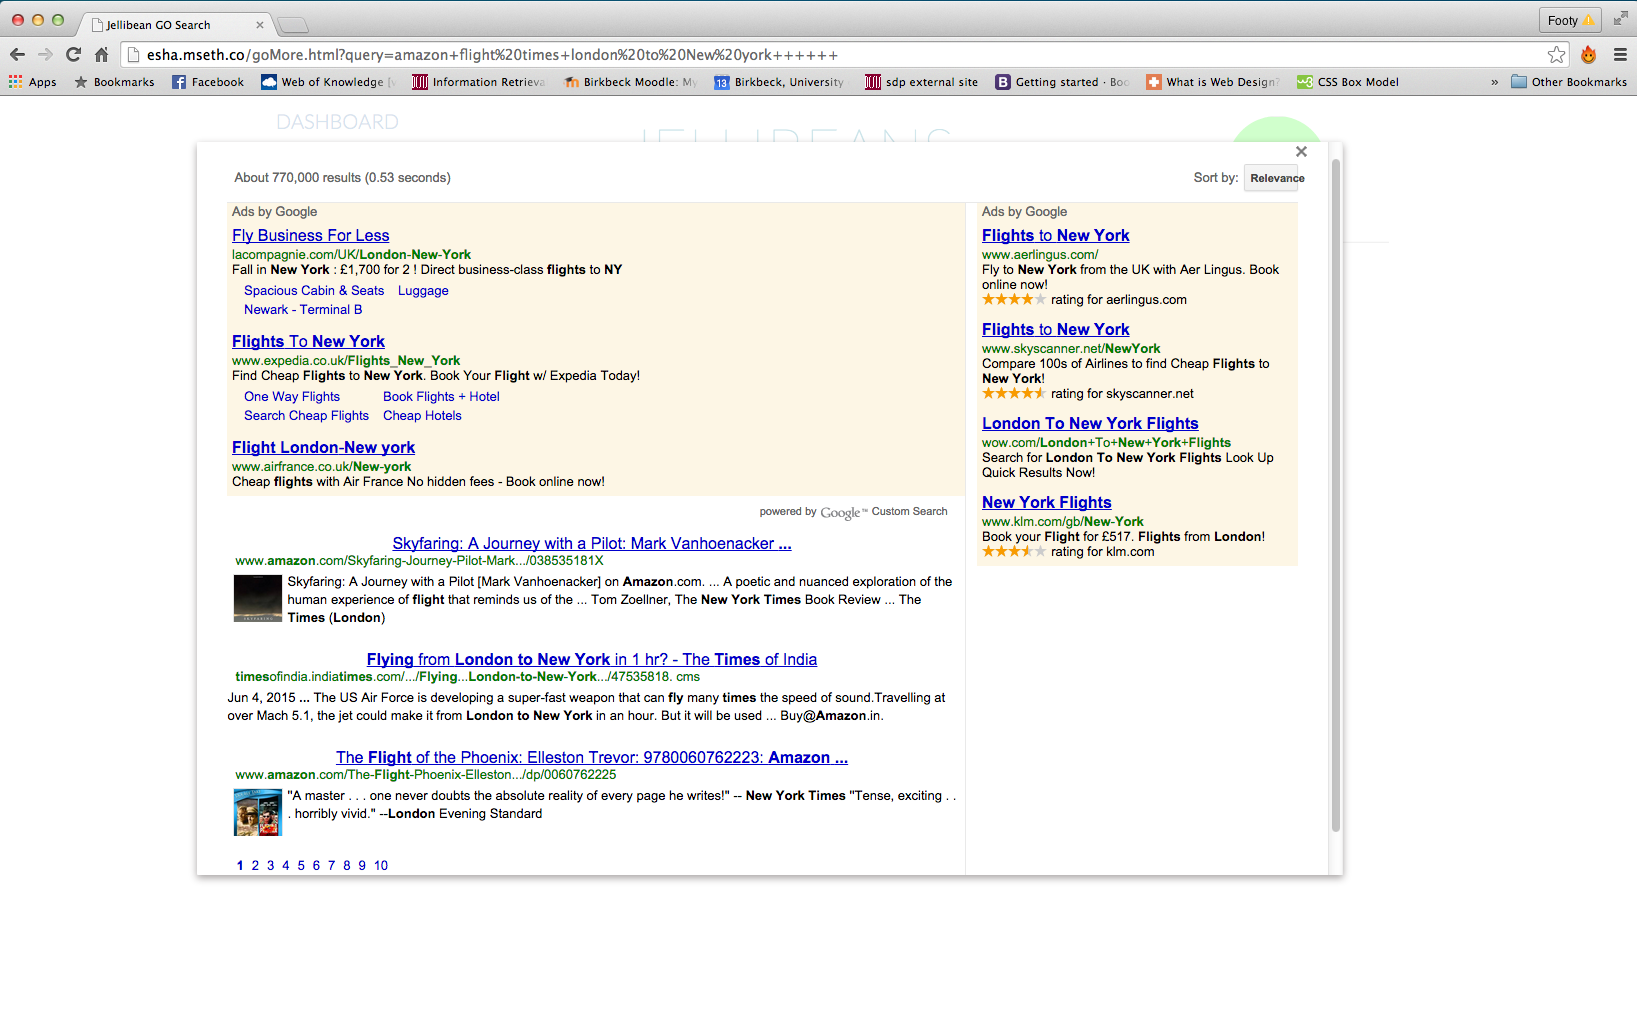
\includegraphics[scale=0.25]{ResultsModal}
\end{center}
\caption{Top 3 results are presented back to users in a modal to reduce information on the page. The modal can easily be closed and reopened.}
\label{resultsModal}
\end{figure}

}
\item{Due to the nature of the parametric search, and the reduction in number of search results displayed, the results from Jellibeans are more likely to be a direct semantic relation to the search query. This makes the selection of that result by the search engine more transparent to the user.}
\item{Integration of the web application with a motion controlled user interface, the LEAP controller.}
\end{enumerate}




\section{Product Specification}
Major dependencies and How I plan on tackling the problem to meet my requirements.\\

The core features for Jellibeans are to implement and test for suitability within an environment for users with Autism are:

\begin{enumerate}
\item{A combination search engine.} \\
A combination search engine that will synthesise the search results from three engines, Google, Bing and Yahoo. The aim of this feature is to increase recall of the engine. 
\item{User Testing.}\\
To test the combination search engine with a sample of users with Autism, and typically developing individuals to ensure that the combination search engine enhances search experience without introducing redundancies. To understand more about the likes, dislikes and preferences of user's self-selected search engines.
\item{User Research.}\\
Research and develop iterations of a \textit{stereotyped} user model of Autism within Search.
\item{Retriving Google+ Data.}\\
To integrate the user model and Jellibeans with Google+, to enhancing the feel of a personalised search engine.
\item{Assessment of the User's Autistic Traits.}\\
To develop a diagnostic assessment page for Jellibeans based on a Psychological assessment, the Autism Quotient \cite{Baron Cohen et al}. Jellibeans will review and assess autistic-like traits or characteristics, so that users can be aware of, and save a copy of their diagnostic information.
\item{Assisting the User to Break Down their Search Query.}\\
To allow the user to navigate Jellibeans to break down their search query into smaller manageable questions to ask, i.e., breaking the query up into `Do', `Know', `Go', `Social' questions.
\item{Parametric Search Process.} \\
To provide a parametric search process, and reduce ambiguity of forming a search query for users with Autism.
\item{Jellibean Suggestions and Assitance.}\\
To provide suggestions or cues for users to assist them with forming a search query, and to help ease some users need of a `perfect' search query.
\item{Prioritising Search Results and Minimising Text Displayed to User.}\\
Jellibeans will prioritise and display the three highest ranking search results for users. The overall goal of this feature is to reduce the amount of text on the page, to minimise the chance of overwhelming users and to retain as high precision of the search results as possible.
\item{User Testing.}\\
To test the \textit{stereotyped} user model embedded within Jellibeans on a sample of individuals with Autism and gather feedback.
\item{Motion Controlled User Interface.}\\
Jellibeans will utilise a motion controlled UI to enhance the search experience for individuals with Autism by making it more receptive and interactive, and to maintain the user's attention for longer.
\item{User Testing.}\\
To gather feedback from a sample of individuals with Autism who have used Jellibeans, and present the findings in the Evaluation and Conclusions (see Section~\ref{eval}).
\end{enumerate}





\section{Software Architecture}

\subsection{Design Patterns}

\begin{enumerate}
\item{Builder Design Pattern.}\\
For Jellibeans to successfully create the user's query string, http GET requests were used to extract parameters from the URL. The Builder Design pattern was used to achieve this. Once the parameters from the URL are retrieved, Jellibeans builds them into the user's search query string. The search query string can then be passed to the JavaScript methods in the relevant class (dependent upon the user's search behaviours), parsed into the correct format, before a POST request is then made to the Jellibeans Custom Search Engine to process the request.
\item{Chain of responsibility Pattern.}\\
Because there are many behaviours that the user can perform before their query string is formulated and ready to be posted to the search engine, the software also makes use of the Chain of responsibility pattern where at each stage the user's query is passed along a chain, with added functionality and methods depending on what the behaviour of the user was.
\item{Adapter Pattern.}\\
I accessed the user's Google+ profile data (name and profile picture) and presented these on the Jellibeans homepage. I then used the Adapter design pattern to build my own functionality onto the existing profile. For example, to present the user's Autism Quotient score, and to guide the user through forming their search query. 
\end{enumerate}


These patterns reduced coupling between the classes and the query, so it was chosen because it follows programming best practice.


\subsection{Use Case Diagram  TODO-redo images}
The main use cases which are required by the Jellibeans application are:


\begin{figure}[H]
\begin{center}
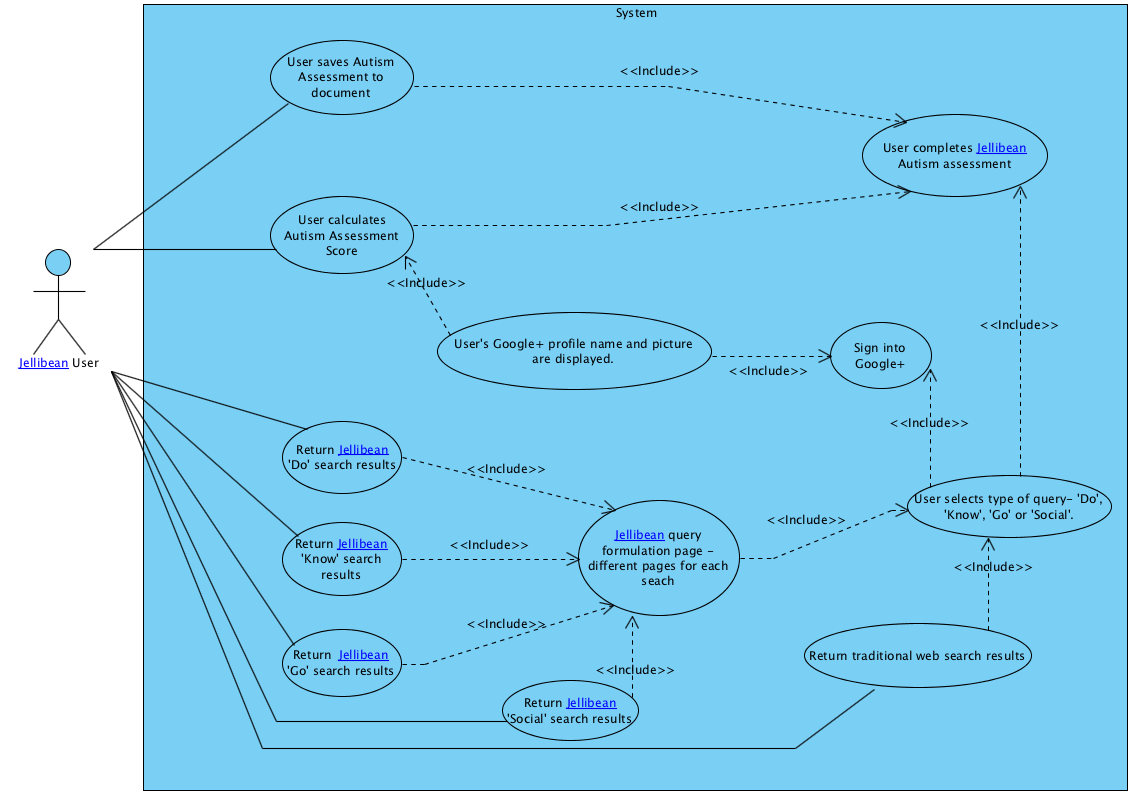
\includegraphics[scale=0.55]{JBeanUseCase}
\caption{Jellibean Feature Uses and High Level UML Use Case Diagram}
\label{JBeanUseCase1}
\end{center}
\end{figure}

\subsection{Class Diagram  TODO-redo images}


\begin{figure}[H]
\begin{center}
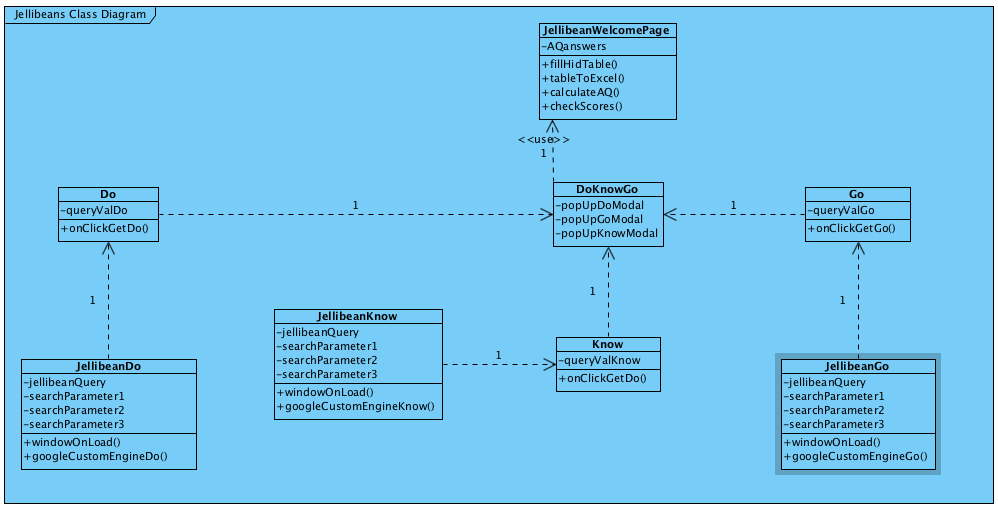
\includegraphics[scale=0.55]{jBeanClassDiagram}
\caption{Jellibean High Level UML Class Diagram of Jellibeans}
\label{jBeanClassDiagram1}
\end{center}
\end{figure}




\section{Implementation}

\subsection{Synthesis of Search Results From Different Engines.}
For search results returned by Google, the Custom Search API was used in line with the Google terms of service, that is that `screen scraping', or copying the data directly from the website is prohibited. The Google Custom Search API is a RESTful API with a single method called list. The API method used was GET, and the response data is returned as a JSON type. The response consists of (1) the actual search result, (2) metadata for search like number of results, alternative search queries, and (3) custom search engine metadata. 

\subsection{JSoup API}
For Bing and Yahoo search results, JSoup (a Java HTML parser) was used to identify the links from the resulting query. The JSoup HTML parser was considered more efficient for retrieving search results, as it could be used to complete the task from both search engines, using a slightly different href element filter for each. JSoup also has advantages over html parsing. It contains a class representing a list of nodes called `Elements', which implements Iterable to iterate over a list in an enhanced for loop.

\subsection{Java}
To test the combined output from the three search engines with a group of users, and gather their feedback on the results, I developed a Java Applet to run the programme (see Figure~\ref{applet}). The search results from the Java Applet were written to a text file.


\begin{figure}[H]
\begin{center}
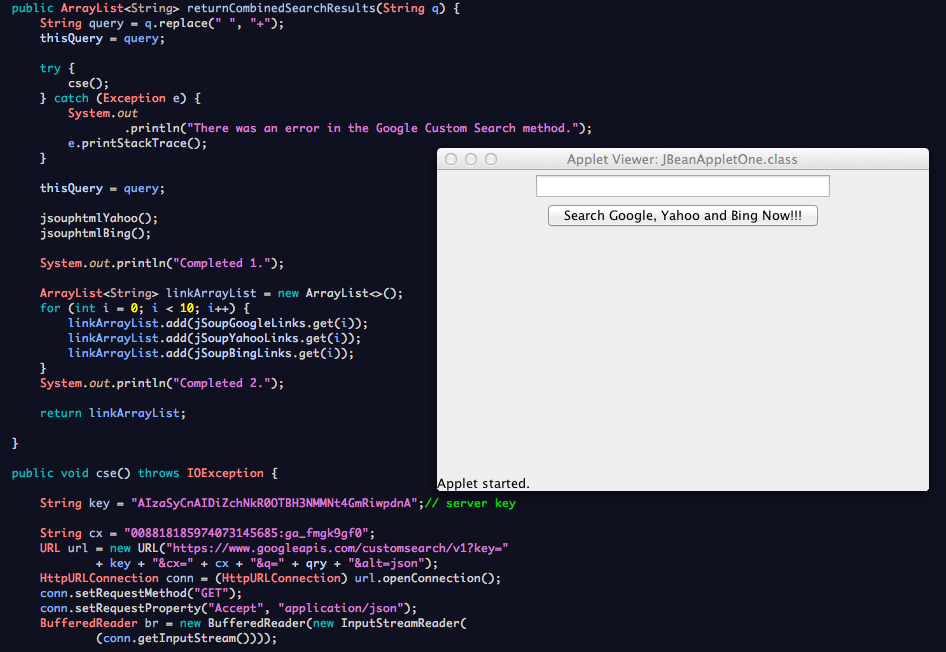
\includegraphics[scale=0.40]{Applet}
\caption{Applet Built to User Test the Combination Search Engine. }
\label{applet}
\end{center}
\end{figure}

Java was chosen for development of `to be tested' packages of features (e.g., the combination search engine). The developer for the project was most proficient with Java, and could quickly develop prototypes for user testing.

\subsection{JavaScript}

JavaScript is commonly used in HTML as it can run locally in a browser (rather than remote server). The Google+ API provided good documentation for using JavaScript. Furthermore the JavaScript code could be easily embedded into the Jellibean HTML code to interact with the Document Object Model (DOM) of the page. The browser was able to respond to user demand quickly, which made Jellibeans more responsive.
\vspace{5mm}
JavaScript was used in this way to return the aboutMe profile information from Google+ to the user.

\vspace{5mm}
JavaScript was also used to calculate the user's Autism Quotient, display the score in the browser, and to save the user's responses to a local Excel file on the users computer so that they can access the data at a later stage.

\subsection{HTTP: Client and Server Set-up}
The Hypertext Transfer Protocol (HTTP) enables communications between web-browsers (clients) and the server (the computer that hosts Jellibeans) using a request-response protocol. Jellibeans was deployed in the web server so that it was ready to be used remotely by users (and for me to gather feedback easily). When the user submits a HTTP request to the server that hosts Jellibeans, it responds with the appropriate behaviour to the client so that the user can formulate their search query and retrieve the results from their search. 

\vspace{5mm}
Jellibeans can be viewed at http://esha.mseth.co.

\subsection{HTML}
HyperText Markup Language (HTML 5) was used to create the webpages for Jellibeans, so that the web browser could render the wesite.


\subsubsection{Bootstrap and CSS}
For front-end development and to style the Jellibean web pages I used the Bootstrap framework \cite{bootstrap} for it's clear styles, good design and ease of use for the current project. I included my own Cascading Style Sheet (css file) where I needed extra styling beyond what the Bootstrap framework could offer. 


\subsection{LEAP motion detector and LEAP SDK}
The LEAP motion controller is a light-weight, portable device that detects user motions using infra-red light. The LEAP has accurate timing, and works well with the combinatorial configuration of senses (sight, hearing and touch). As this is a tool to be used with individuals with Autism, who have increased sensitivity to touch, the LEAP is the perfect choice as there is no additional sensations to the users body. The LEAP is affordable for users to integrate with search at home, and currently retails for about £60.

\subsection*{TODO}
API's and Development Tools\\
Describe the technologies used in the project, why they where
chosen and what were the other options:\\
Tools and programming languages\\





\section{Software Development Process}
\subsection{Core Feature 1: Research and Data Collection for a Combination Search Engine using Google, Yahoo and Bing.}

To implement the combination search engine I used three API’s provided by Google, Bing and Yahoo, namely, the Google Custom Search API, Yahoo BOSS Java API and Bing Search API. 
\vspace{5mm}
To get started with the Google Custom Search API, I created a project called \textit{Jellibeans} in the Google Developers Console, and an OAuth 2.0 Client ID. I obtained a Consumer Key and Secret to use the API, and used these in the application code to access the Google Custom Search Engine (see Figure~\ref{JBeanAppletGoogleCustomSearch1}). 

\begin{figure}[H]
\begin{center}
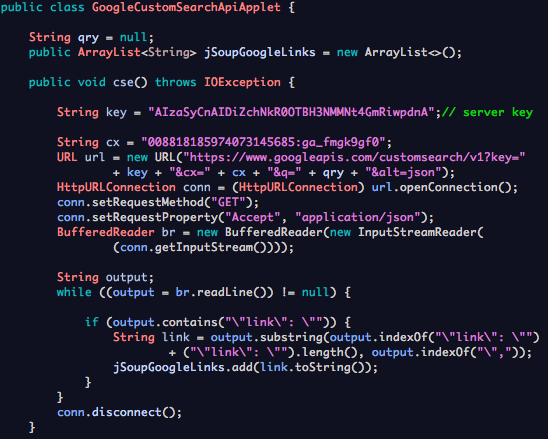
\includegraphics[scale=0.7]{JBeanAppletGoogleCustomSearch}
\end{center}

\caption{Jellibean Applet Combination Search Engine}
\label{JBeanAppletGoogleCustomSearch1}
\end{figure}

Following that I also registered my JavaScript origins within the console to access the Google+ API, and redirected URIs so that once users sign in using their Google+ login credentials they will be redirected to Jellibeans (or http://esha.mseth.co). This was done because I wanted users to be able to sign in and access their google profile from Jellibeans (see Figure~\ref{GoogleSignInPage}). 

\begin{figure}[H]
\begin{center}
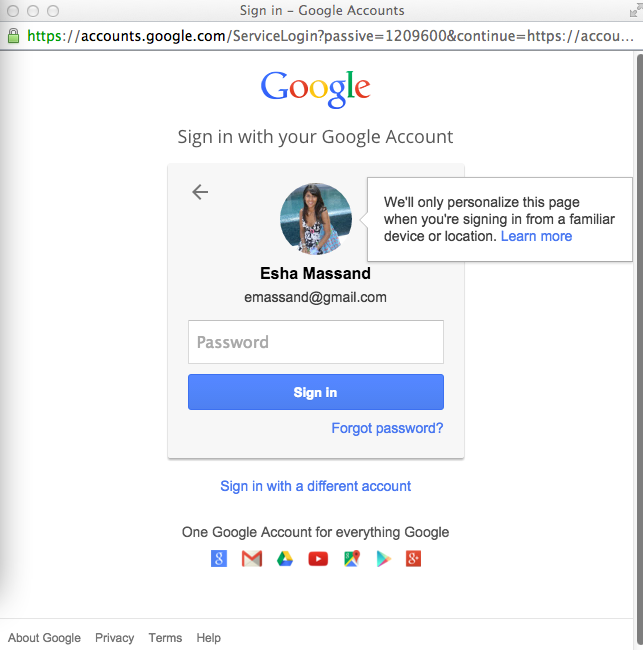
\includegraphics[scale=0.3]{GoogleSignIn}
\end{center}
\caption{Google Sign In Page.}
\label{GoogleSignInPage}

\end{figure}

Following a similar protocol for Yahoo and Bing Search API’s, I created projects in the Yahoo Developers Network, and Microsoft Azure Marketplace, and purchased an API Consumer Keys and Secrets (needed to use the APIs). 

\subsubsection{Web Scraping}
Web scraping was also an option, it quickly became a preferred because of integration of the three API’s and the flexibility/manipulation of  the results if they were returned using the same method. However this was against terms of service set out by Google (see section 5.3 of Figure~\ref{GoogleToS1}).

\begin{figure}[H]
\begin{center}
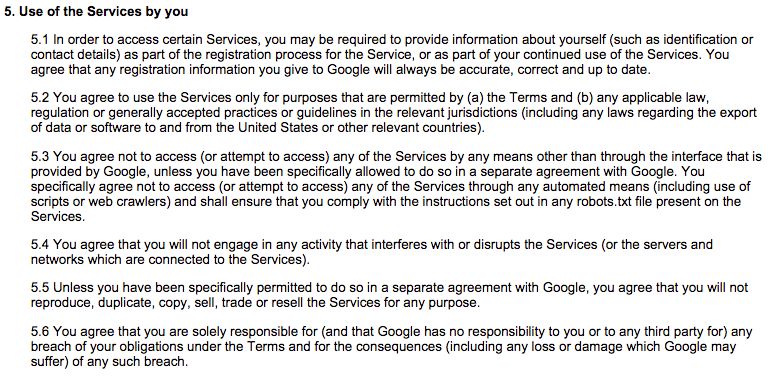
\includegraphics[scale=0.6]{GoogleToS}
\caption{Google Terms of Service}
\label{GoogleToS1}

\end{center}
\end{figure}


So, instead, I used the Jsoup API \cite{jsoup}, which is a java –written API for HTML. The library provides methods to conveniently extract data using DOM (Data Object Model) and CSS (Cascading Style Sheet) methods. The Jsoup HTML parser was used to scrape results only from Yahoo and Bing, and integrated these into a Java Applet that runs in Eclipse Luna IDE (see Figure~\ref{AppletFig}). The top 10 links, from each search engine were presented to users and ranked such that result 1 from Google was followed by result 1 from Yahoo, and that was followed by result 1 from Bing. Then results 2 from Google, Yahoo and Bing were presented and so on, until the 30 links were produced, in ranked order from the three search engines. 

\begin{figure}[H]
\centering
\begin{subfigure}{.5\textwidth}
  \centering
  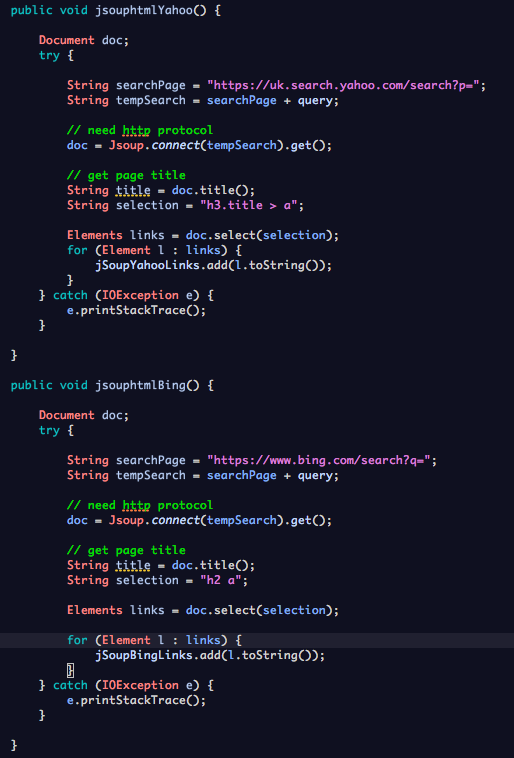
\includegraphics[width=.7\linewidth]{htmlParsers}
  \caption{JSoup HTML Parser.}
\end{subfigure}%
\begin{subfigure}{.5\textwidth}
  \centering
  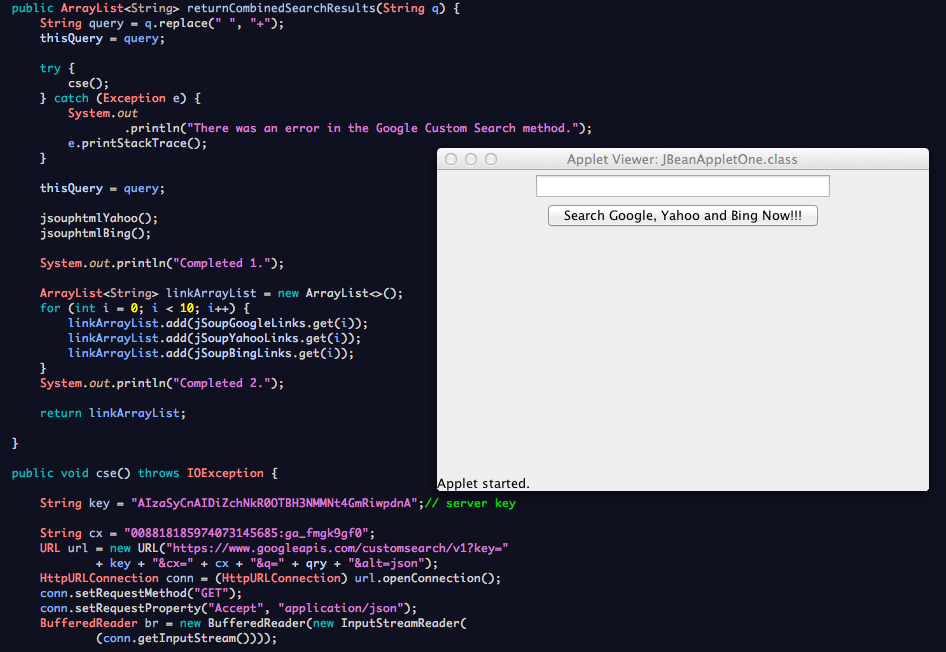
\includegraphics[width=.7\linewidth]{Applet}
  \caption{Complete query results.}
\end{subfigure}
\caption{JSoup HTML Parsers for Yahoo and Bing working with Google Custom Search API in Java Applet for testing.}
\label{AppletFig}
\end{figure}

\subsubsection{User Research and Testing of Core Feature 1}
To test the integrated combined search engine, the returned documents from 10 pre-determined search queries were presented to 10 participants who were identified as high AQ scorers. Participants were asked to comment on the search results that had been returned, and to choose three out of the links returned to follow up with, and to observe if anything was odd about the results returned. The responses from the 10 users were analysed to test core feature 1 and whether a combination search would be a good option for Jellibean Search, or whether it would introduce redundancy in the search results. 
\vspace{5mm}
Somewhat non-surprisingly (given the statistics of preferred search engines) the results revealed Bing Search was favoured the least, and Google results the most, with Yahoo falling somewhere in between. Out of the 30 responses participants indicated to follow up with, 21 were Google results, 3 were Yahoo, and 1 was Bing and 5 results overlapped between Google and Yahoo.
4 participants commented that the Bing results were distracting rather than helpful.
\vspace{5mm}
Given these findings from the user group, it was decided to continue using the Google results, but to drop the results from Yahoo and Bing, in line with the aim of the project as a whole – to improve returned search results for users with Autism.



\subsection{Core Feature 2: Building a User Model of Autism.}
To identify the features of the user model to build, I ran a study to collect example search queries on a set of informational needs from 37 participants. The participants were asked to give examples of search queries they would use to identify the name of a song they had heard (given the lyrics), or the name of a breed of a dog they had seen (given a picture of the dog). There were in total 10 search queries; the study was distributed widely via Surveymonkey.com \cite{surveymonkey} and can be seen in Appendix ~\ref{AppendixA}. Participants were also asked to complete the Autism Spectrum Quotient 50-item questionnaire see Appendix ~\ref{AQ}. The participants responses are analysed and reported back to surveymonkey.
\vspace{5mm}
The range of scores for the AQ is 0 to 50 with high scores indicating increased likelihood of autism-like traits. A score under 21 is a low to average result (many women average around 15 and men around 17). A score of 22-25 indicates autistic tendencies slightly above the population average. A score above 26 gives a borderline indication of high functioning autism, or Aspergers. A score above 30 suggests a likelihood of Aspergers syndrome or autism (sensitivity of test measure = 79\% \cite{Baron Cohen et al}).For the purposes of this study, individuals with scores equal to, and above 30 were interpreted as having `autistic-like traits'.
\vspace{5mm}
Participants were divided into two groups; low AQ scorers (scores below 30), and high AQ scorers (scores equal to and above 30). There were 30 low AQ scorers and 7 high AQ scorers. 


\subsubsection{Differences in Search Queries Between Users With and Without Autistic-like traits.}
I conducted a qualitative analysis on the search query strings from both low and high AQ scorer groups.
\vspace{5mm}
In both groups, Google was the prefered search engine by far, with all participants reporting that they used Google as a first choice. No one in the current sample used Yahoo or Bing. 
The low AQ scorer responses were analysed as a group. A baseline answer was generated using a frequency criterion of 40\% i.e., if 12 out of 30 respondents or more generated the same query string given an informational need, it was included in the model below. If two responses were equally as common, both are reported in the model. Data was discarded when a response indicated that the participant would do an image search, as this was not the aim of the survey. The results from the frequency analysis are presented below.

\begin{enumerate}
\item{You hear a song on the radio with the lyrics, `Look at your children', and you want to download it. What would you type into search on your favourite search engine to find out what song it was?\\\textit{Look at your children song}. \\\textit{Look at your children lyrics}.}
\item{You've lost touch with an old school friend (you went to St. Mary'€™s School). What key words/queries would you use to find them?\\\textit{St. Maryâ€'s School Year of X}.}
\item{How would you identify what this is using a search engine (pretend you don'€™t know what it is called). What key words/queries would you use?\\\textit{Star shaped brown plant}.}
\item{How would you find out the name of this famous person using a search engine? What key words/queries would you use?\\\textit{Brown hair famous young women}.}
\item{How would you identify what breed this animal is using a search engine? What key words/queries would you use?\\\textit{Small dog fluffy breed}.}
\item{Your friend and you can'€™t agree on how Thandie Newton pronounces her first name. How would you resolve this using a search engine?\\\textit{Thandie Newton pronunciation}.}
\item{What would you search for to identify this pattern'€™s name, and which country it originates from?\\\textit{Repeating square maze pattern border}.}
\item{How would you search for delay'€™s relating to your (imminent) flight to Paris?\\\textit{Flight number, carrier, Paris, airport, flight time}.}
\end{enumerate}

The following observations were made for the users in the high AQ group:
\begin{enumerate}
\item{There were an increased number of incompletely-formed queries. In the high AQ group, participants were more likely to miss off words in the query string. This was observed even though the sample size was much smaller in the high AQ group (7 people) compared to the low AQ group (29 people)). For example, when analysing the results from query 1 above, 2 out of 7 respondents in the high AQ group did not put `lyrics' or `song' in the search query when searching for the lyrics ``Look at your children". When these search strings are entered into Google, the results are very different (see Figure~\ref{someresults}). More results are returned to the incomplete query (302,000,000 compared to 32,900,000). The high AQ user group are presented with results that have a lower precision, i.e., more irrelevant information that they must sift through to find the answer to their search query.}
\label{incomplete}


\item{Although many high AQ scorers' formed query strings well, there was increased use of idiosyncratic words in the query strings that were formulated. This is in line with previous research that suggests that people with autism organise information in more subjective and individual ways \cite{subjective organisation}. For example, referring to the picture of the dog as `yorkie pooh'(not listed in frequency index), `aeroplane' (frequency of 8254 words per million) instead of plane (frequency of 33900 words per million) or flight (29535 words per million) , `miniature' (less than 4973 words per million) instead of small (185463 words per million). The idiosyncratic nature of the words is captured by their lower frequency of use in the English language. Search engines use term frequency to determine if a document is relevant to the users search query. If the frequency of words used to form search queries differs between low and high AQ scorers, so will the rankings of the returned search results.}
\label{idiosyncrasy}

\begin{figure}[H]
\centering
\begin{subfigure}{.5\textwidth}
  \centering
  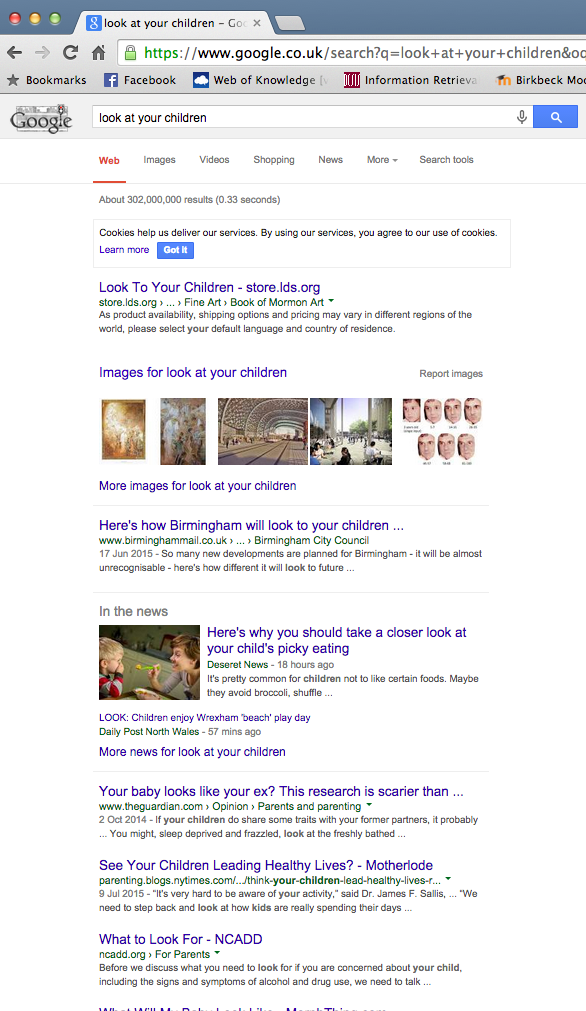
\includegraphics[width=.7\linewidth]{lookAtUrChildren}
  \caption{Incomplete query results.}
\end{subfigure}%
\begin{subfigure}{.5\textwidth}
  \centering
  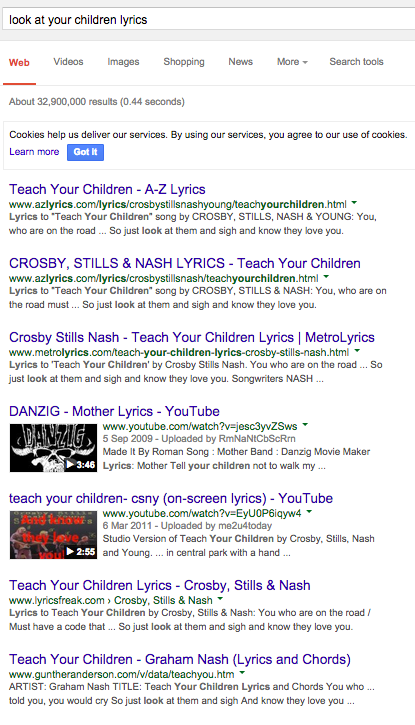
\includegraphics[width=.7\linewidth]{lookAtUrChildrenLyrics}
  \caption{Complete query results.}
\end{subfigure}
\caption{High and low AQ scorers both formed search queries accurately, however there was an increased tendency to omit the word ``lyrics" in the high AQ group resulting in very different search results.}
\label{someresults}
\end{figure}

\begin{comment}

\begin{figure}[H]
\begin{center}
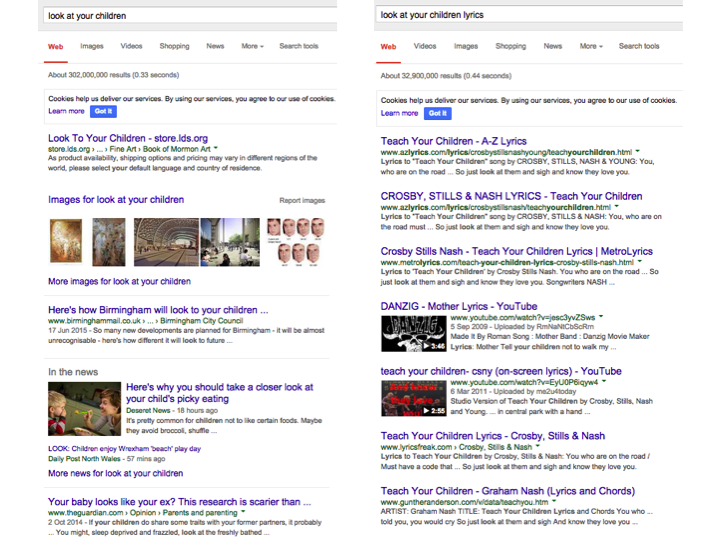
\includegraphics[scale=0.5]{LookAtYourChild}\\
\label{LookAtYourChild}
\end{center}
\end{figure}

\end{comment}


\item{One individual of the 7 individuals in the high AQ group demonstrated ambiguous use of third-person pronouns, which is characteristic of some individuals with Autism \cite{pronoun}. This includes using first names. This is particularly detrimental to search engine query strings because the use of names disrupts the term frequency - inverse document frequency weighting \cite{tfidf} of the search query and subsequently the results returned to the user.
}\label{pronoun}
 
\item{
For questions that were `social' in nature (e.g., featuring a face of a famous woman), 2 out of 7 individuals in the high AQ group indicated that these were types of queries that they would not normally be interested in, and so ``wouldn't bother asking it". This is, of course, in line with the characteristics of Autism according to \cite{DSM}. For these queries, it was more common for individuals in the high AQ group to include information in their search query string that was extraneous to the search question itself, compared to the low AQ group. For example, in query 4 above (which asked respondents to indicate how they would identify a famous person), 2 high AQ scorers included information about the woman's earring. Inevitably this `dilutes' the search query and results in reduced precision for the search engine.
}

\begin{comment}
\item{ 
Lastly there were more spelling errors and typographical errors in the high AQ group compared to the low AQ group.
}\label{spelling}
\end{comment}



\end{enumerate}


\subsection{Core Features 3 and 4: Jellibeans -- Transforming the User Query.}
Given the set of observations in the data reported above, the aims were to devise a set of rules that would `transform' queries made by individuals in the high AQ group to those similar to the low AQ group. The search engines already handle some of the observations from high AQ scorer queries. For example, the use of pronouns ('I' and `You') is already taken care of with the use of stop words, which is implemented by the search engine itself. The aim of the project is to therefore address issues that result in the search query string being misleading, and returning differnt results to low AQ scorer search queries. 
\vspace{5mm} %5mm vertical space

The aim for Jellibeans is to return search results that are more in line with low AQ scorers. In other words, search results from high AQ queries shared greater overlap with those made by the low AQ group, even though the queries were formed differently. The rule engine is thus a concrete and operationalised framework, for a theoretically-grounded user model of autism within search. \\

\vspace{5mm} %5mm vertical space
Jellibeans works to address more than one observation made during the data collection stage. As a general rule, changes will take the form of add on questions that aim to structure the individual to form a search query in a logical order so that key search terms are not dropped. The structure of the query's formation should also assist the user with less idiosyncratic search queries. \\


\vspace{5mm} %5mm vertical space

To address observation \ref{idiosyncrasy} and to make high AQ scorer search queries less idiosyncratic, Jellibeans will prompt the user to categorise their search query into one of 4 possible types of queries, a `DO', `Know', `Go' or `Social' query. Each type of query will be associated with a colour, and this colour will be prominent on the page, to serve as a visual reminder of the task. This works to reduce the working memory load for the user, and to serve as a goal-directed cue -- two things we know are difficult for people with Autism are maintenance of information in working memory, and goal-directed tasks involving a high demand on Executive Functioning (Executive functions (also known as cognitive control and supervisory attentional system) is an umbrella term for the management (regulation, control) of cognitive processes, including working memory, reasoning, task flexibility, and problem solving as well as planning and execution \cite{EF}.) 

\vspace{5mm} %5mm vertical space

The Jellibeans `Social' query applies particularly to the user group in question. Social queries specifically help users when performing a social search, for example when they are looking for a person on the web. The social page has hints and suggestions that can be added into search to assist the user with cues that may be helpful for their search, and to improve search results that are returned from Jellibeans.

\vspace{5mm} %5mm vertical space
To address observation \ref{incomplete}, Jellibeans will have a `search display' box that shows the user exactly what will be searched for, and also works to train the user in the long term about how to form a search query string. Because the current research identified that user's with Autism formed search queries were particularly incomplete for socially-grounded informational needs, extra functionality has been added to the `Social' query page. For example, when the user is completing `Social' search parameters, they will be prompted to make additional selections, e.g., if the user has indicated that they are searching for a famous person, they will be prompted for descriptions about that famous person's personality and character (amongst other things). This would ensure user search queries are more complete than they otherwise would have been.

\begin{figure}[H]
\begin{center}
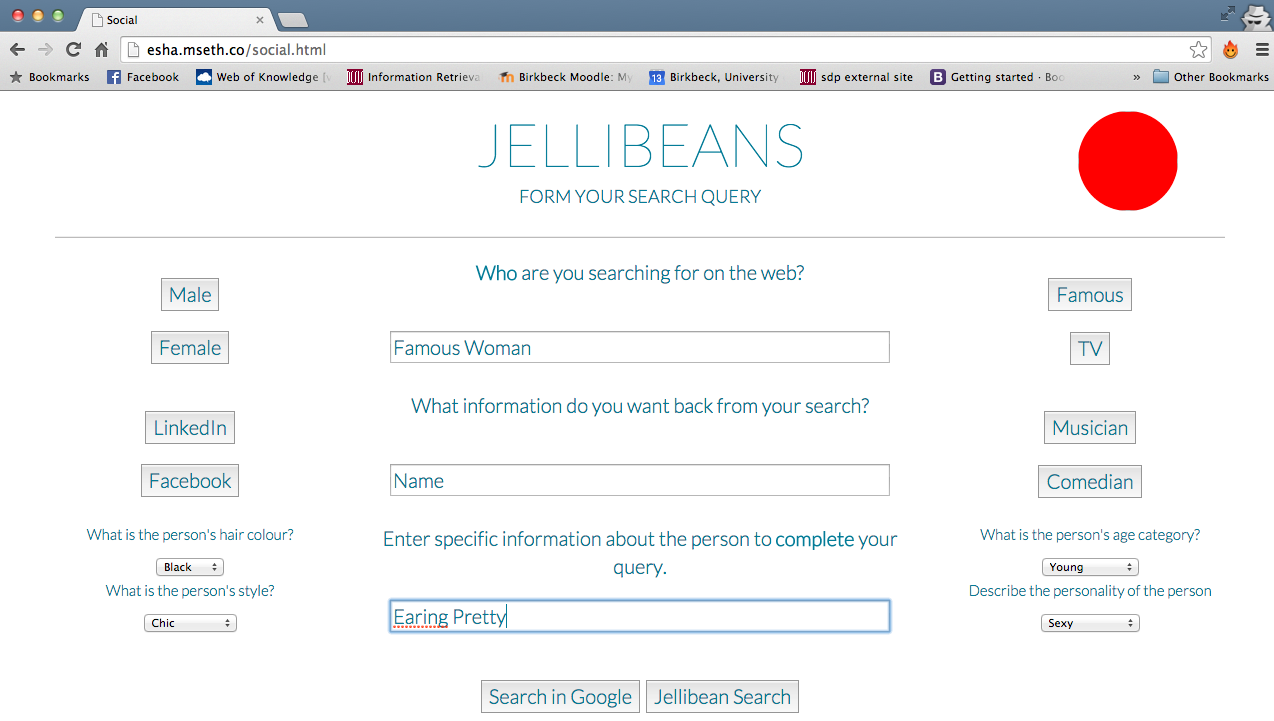
\includegraphics[scale=0.3]{SocialCompleted}
\caption{Example of User's Social Search in Jellibeans.}
\label{socialCompleted}
\end{center}
\end{figure}


\vspace{5mm} %5mm vertical space
For observation \ref{pronoun}, pronouns (`I' and `You') are ignored via a stoplist which is implemented by the search engine itself. Jellibeans will also identify names of people via the third person library and suggest that these are removed, replaced with another search query term, or kept if the keyword is relevant. The extra layer of checking refines the search query.

\begin{comment}
\vspace{5mm} %5mm vertical space
Because Jellibeans bypasses the search engine interface, a spell checker will be implemented to address increased spelling errors in high AQ scorers (observation \ref{spelling}). This will also be in the form of a `suggestion' at the search query formulation stage.

\end{comment}

\vspace{5mm} %5mm vertical space

The Autism Quotient score of the user will be stored.


\subsection{Core Feature 5: Integration with a Motion Controlled Interface.}
Integrating Jellibean with Motion Controller Hardware
LEAP motion controller and its use for the system.
Current Project's Hardware Selection Process and Important Design Issues:
\begin{enumerate}
\item{Good timing correlates to a good meaning and User Experience.}
\item{The leap has options to poll frames at a constant rate (to keep timing of movement accurate) which is important.}
\item{Cognitive lag time. Each of our senses operates with a different lag time. Hearing has the fastest sense-to-cognition/understanding time, and surprisingly sight -- the slowest. If the devices interferes with the processing of the sense, it will confuse the combinatorial configuration of the senses, leading to misunderstandings in the meaning and a worse user experience.}
\item{Volume is important because this is a tool to be used with individuals with ASD, the device must have a low volume€™, i.e., the sensory experience cannot be overwhelming.}
\item{Load, by this I mean `cognitive' load is most desirable when not high. We do not want the device to be overwhelming in terms of it's cognitive load.}
\item{Within the selection process, I did not just consider the physical design of the device, but also the way in which the devices manifests actions into behaviours. That is, how does the user engage behaviourally within the environment using the device? What about the physical sensation and its path towards a behavioural or emotional response? For example, can we program there to be an activity followed by a reward to reinforce the activity.}
\end{enumerate}

\subsubsection {Evaluation and Review of the Leap Motion Controller.}
Advantages
\begin{enumerate}
\item{Impressive}
\item{Uses infrared to embed the users (phantom) hand on the screen}
\item{New technology and novel to bring to laptops}
\item{East to set up}
\item{Has built in gestures and navigation tools}
\item{Can work in pretty dimly lit environments (but not all)}
\item{It is sophisticated (sometimes the polling frequency lets it down)}
\item{Picks up an impressive distance along the z axis}
\item{Offers a recalibration process if the controller is persistently jumpy, or there are discontinuities in the tracking data, if there are aberrations in the tracking data that occur in certain areas of the field of view, or poor tracking range. This can be done using the shiny surface such as the computer screen or mirror.}
\end{enumerate}	
Disadvantages
\begin{enumerate}
\item{Misses small hand movements}
\item{The range that it will detect is 150 degree angle along the y axis, this is reasonable but not always idea when gestures/hand movements are large.}
\item{Some parts of the screen the hands to not ‘reach’, i.e., bottom left /right of screen are sometimes hard to reach.}
\item{Loses the hand, stops working/sensing the hands, even when the controller stays on.}
\item{Often misses frames, so the user makes larger hand movements and then overshoots (when the LEAP catches up)}
\item{Built-in controls are not ideal}
\item{Lighting works best when the hand is seen in silhouette fashion by the controller. }
\end{enumerate}

\section{Software Testing}

The JavaScript Console was used for testing JavaScript code. \cite{javascripttesting}, I also used JSfiddle \cite{jsfiddle} to ensure the code contained no bugs, and was particularly good for seeing how the JavaScript code integrated with the HTML code and CSS.

\vspace{5mm}
JUnit was used to test the Combination Search Engine, which was written using Java code. Unit testing was completed, mostly at the method level.

\section{User Verification and Testing}
Five high AQ scorers were called back for interviews and a focus group. During the interview, individuals were given the same user search queries as in the data collection and research phase of the study. For each transformation that was implemented, users were asked to comment on whether it enhanced or took away from the ease of their search experience, and from their satisfaction with the search results. Users were asked to comment on:
\begin{enumerate}
\item{Whether they liked the parametric search style of Jellibeans}
\item{The `narrowing' the scope for irrelevant detail, with more concrete questions above the search bar}
\item{Why they may choose Jellibeans over other search engines, for example, Google}
\item{The speed and efficiency of search with Jellibeans}
\item{The search query results themselves}
\item{The display and layout of the results}
\end{enumerate}

\subsection{The positives}
Users verified that the `Dashboard' colour coding was helpful (see Figure~\ref{colourCoding}). The colour of the chosen type of search remained on screen for its duration.

\begin{figure}[H]
\begin{center}
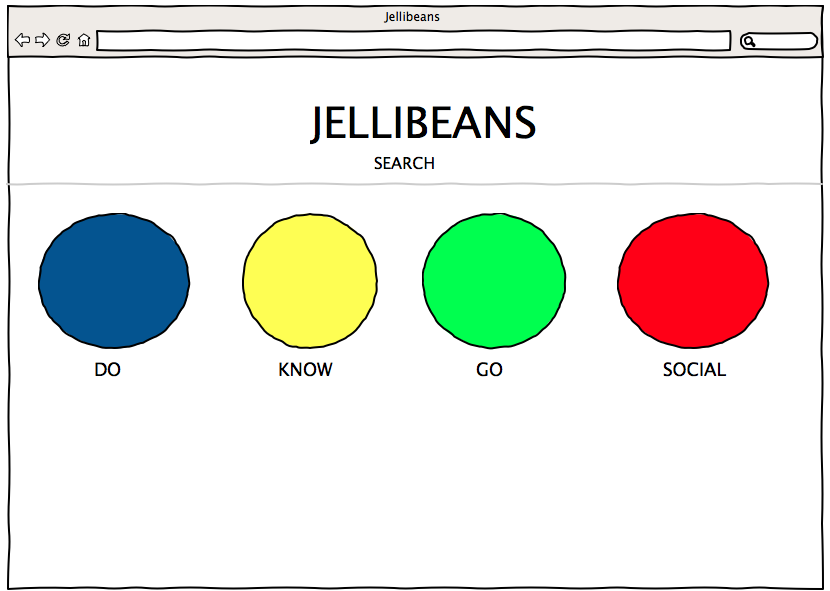
\includegraphics[scale=0.25]{DoKnowGoSocial}
\caption{Colour coding on Jellibean dashboard.}
\label{colourCoding}
\end{center}
\end{figure}

The modals (floating window reminders) for each of the colour themes were useful for newer users, when they were unfamiliar with the colours. The associations for all user groups, including users with Autism, were quick to learn, these were single link visual (rather than verbal) associations.\\

\vspace{5mm}
One tester with high functioning Autism described that the direct question (i.e., `What do you want to do on the web?'), with suggestions (`Shop', `Watch', `Listen'), was useful when he was ``at a total blank". He disclosed that often his need for perfectionism and sameness could have him staring at a blank screen until he came up with the `perfect' query. However, the suggestions were helpful for him to get started, and so his experience was that the queries were completed faster than usual.  \\

\vspace{5mm}
During the focus group, participants agreed that one of the major positives of Jellibeans was that unlike Google, users did not receive back hundreds and thousands of mostly irrelevant results. Jellibeans held their interest for longer because of the reduced number of results that users had to sift through. Testing also revealed that the parametric search style meant that they did not need to try and remember all the key words to search for, rather the cues helped them remember points they would have missed otherwise. \\

\vspace{5mm}
Another common comment was the time/reward payoff from completing a detailed search form. Users agreed that although they would spend more time formulating their search query, they were likely to save time that would usually be spent sifting through search results.\\

\vspace{5mm}
All users positively commented on the reduced number of search results presented (top 3). The amount of textual information that was presented back on the results page is significantly reduced in Jellibeans. 


\subsection{The negatives}

One comment during the first iteration about Jellibeans was that the results were not specific enough to the search, and that a better precision needed to be achieved. To increase the precision of the engine, Jellibeans implemented `AND' boolean operators between each input of the parametric search. This increased precision significantly, and recall dropped. However it led to a better user experience than without this modification.

\vspace{5mm}
One participant commented that the suggestions on the `Do', `Know', `Go' and `Social' pages were not user-specific (see Figure~\ref{suggestions}). 

\begin{figure}[H]
\begin{center}
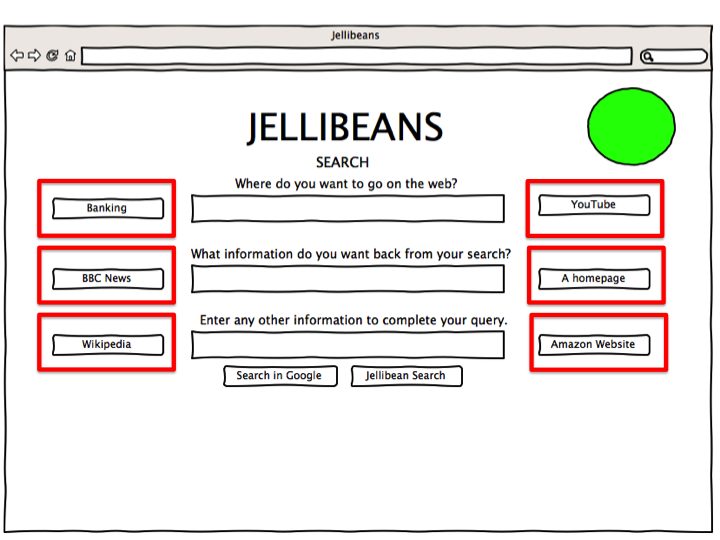
\includegraphics[scale=0.3]{suggestions}\\
\caption{Suggestions on Jellibeans `Go' page for users to help with search query formulation (suggestions are highlighted in red).}
\label{suggestions}
\end{center}
\end{figure}

He suggested implementing something that is user-centred, or, trending, rather than static, as these may not be suited for all users. However, one of the aims of the current project was to reduce the restricted and repetitive nature of search queries for people with Autism. One future suggestion for Jellibeans in order to achieve a balance between user-specific suggestions but not restricted interests, is to include a recommendation system that change often enough for them not to be repetitive. 

\vspace{5mm}
One (possible) negative that was identified with Jellibeans was that the time/reward payoff is really only apparent, over and beyond a traditional search engine, when the search query is complex, or if users are searching for something they have yet to identify, or something ambiguous. To overcome this criticism, Jellibeans includes a `Search in Google' option, so that if users know what they are searching for, they have the option to run the search outside Jellibeans.

\vspace{5mm}
Describe the verification process you used in your project\\
Unit Testing, Static Analysis for methods in javascript etc.\\
Manual testing, Selenium, Cucumber etc for html.\\
Regression tests


\section{Evaluation and Discussion.}\label{eval}

\begin{comment}
The final section summarises the project as a whole
A critical evaluation by the student, emphasising
strong points and weak points
lessons learnt
design decisions which, looking back, would be made differently
ways in which the project could be improved or extended etc.
recommendations for the project
You can also describe possible future work in the area of your project
\end{comment}



Robots
Apache Lucene
Sandboxes
JavaScript html can't access third party pages
Yahoo and Bing was easier and faster to do html scraping


How does it compare to the original specification
This work has successfully completed aims XXX

The final section summarises the project as a whole\\
A critical evaluation by the student, emphasising\\
strong points and weak points\\
lessons learnt\\
design decisions which, looking back, would be made differently\\
ways in which the project could be improved or extended etc.\\
recommendations for the project\\
You can also describe possible future work in the area of your project

\subsection{Signals of Quality Content}
I will test and evaluate the system. Testing will involve assessing the reliability and robustness of Jellibeans; the ease of its interaction; boundary conditions; ease of use; does it fulfil the aims of the project.
Evaluation of the system will include comparisons to existing search engines; assessing how this idea can be implemented to tailor an existing systems; assessing how well the system does compared to existing systems on a set of criteria that are only relevant to the user group in question (a collective measure of user happiness). Evaluation will also include quantitative metrics such as Recall, Precision, and False Negative/Positive rates.


Apache Solr\\

\subsection{Future Directions}
Future directions for the current project would be to develop an API or library for word frequencies in the written English language. These frequency data could have been used to suggest words that were more frequent in the written language for people with Autism, who tend to use idiosyncratic language. This would suggest alternatives for the user.\\

\vspace{5mm}
Alternatively, to use a thesaurus in the current project would be a useful addition.\\

Maybe google which has access to current trending searches would be able to have the `floating' modals to reflect the trends but the current version of Jellibeans is a working example of what could be achieved but with searches that are generally common, rather than trending.

\vspace{5mm}
colour blindness considerations - accessibility for people with Autism  



\clearpage
\begin{thebibliography}{100}
\bibitem {adam}Lella, A., (2014). \textit{comScore Releases March 2014 U.S. search Engine Rankings.} ComScore.com. Retrieved 21 Feb 2015
\bibitem{Baron Cohen et al} Baron-Cohen, Wheelrigjt, Skinner, Martin, Clubley (2001).  The Autism-Spectrum Quotient (AQ): evidence from Aspergers Syndrome/high-functioning autism, males and females, scientists and mathematicians.  \textit{Journal of Autism and Developmental Disorders, 31}, 5-17.
\bibitem{bootstrap}Bootstrap, http://getbootstrap.com/ Retrieved September 2 2015
\bibitem{attention} Bronwyn, M, Murray, M, and Durkin, K. (2003) Weak central coherence, poor joint attention, and low verbal ability: Independent deficits in early autism. \textit{Developmental Psychology, 39}, (4), 646-656. http://dx.doi.org/10.1037/0012-1649.39.4.646
\bibitem{subjective organisation} Bowler, D. M., Gaigg, S. B., Gardiner, J. M. (2008). Subjective organisation in the free recall learning of adults with Aspergers syndrome. \textit{Journal of Autism and Developmental Disorders, 38}(1), pp. 104-113. doi: 10.1007/s10803-007-0366-4 
\bibitem {CDC}Developmental Disabilities Monitoring Network Surveillance (2010) \textit{Centers for Disease Control and Prevention (CDC). Prevalence of autism spectrum disorders: Autism and Developmental Disabilities Monitoring Network, United States. MMWR Surveill Summ.2009; 58},
\bibitem {DSM}Developmental Disabilities Monitoring Network Surveillance (2010) \textit{Centers for Disease Control and Prevention (CDC). Prevalence of autism spectrum disorders: Autism and Developmental Disabilities Monitoring Network, United States. MMWR Surveill Summ.2009; 58}, 10:1–20
\bibitem{EF} Executive Function, https://en.wikipedia.org/wiki/Executivefunctions, Retrieved 27 August 2015.
\bibitem{disengagement}
Elsabbagh, M., Volein, A., Holmboe, K., Tucker, L., Csibra, G., Baron-Cohen, S., Bolton, P., Charman, T., Baird, G. and Johnson, M. H. (2009), Visual orienting in the early broader autism phenotype: disengagement and facilitation. \textit{Journal of Child Psychology and Psychiatry, 50}, 637–642. doi: 10.1111/j.1469-7610.2008.02051.x
\bibitem{seo} Fishkin (2015) https://moz.com/beginners-guide-to-seo/how-people-interact-with-search-engines, Retrieved 3 August 2015.
\bibitem {gameshealth} Games for Health (2012) \textit{Screen-based technologies and Autism. 1}: 248-53
\bibitem{leap} Leap Motion, \textit{Java SDK Documentation}, \\https://developer.leapmotion.com/documentation/java/index.html Retrieved 1 April 2015.
\bibitem{motioncontrollerforautism} Garzotto, F., Valoriani, M. and Bartoli, L. (2014), Touchless Motion-Based Interaction for Therapy of Autistic Children, Virtual, Augmented Reality and Serious Games for Healthcare, \textit{Intelligent Systems Reference Library, 68}, 2014, pp 471-494
\bibitem{googleTerms} Google Privacy and Terms, http://www.google.com/policies/technologies/, Retrieved 27 August 2015.
\bibitem{javascripttesting} JavaScript Console, https://developer.chrome.com/devtools/docs/console, Retrieved September 3 2015.
\bibitem{jsfiddle} JS Fiddle, https://jsfiddle.net/, Retrieved September 3 2015.
\bibitem{jsoup} JSoup Java API, http://jsoup.org/, Retrieved 27 August 2015.
\bibitem{mottron}Laurent Mottron, Jacob A. Burack, Johannes E. A. Stauder, Philippe Robaey (1999) Perceptual Processing among High-functioning Persons with Autism. \textit{Journal of Child Psychology and Psychiatry 40}, (2), 203211. doi:10.1111/1469-7610.00433.
\bibitem{moore}Moore, D. J., McGrath, P., \& Thorpe, J. (2000). Computer aided learning for people with autism—a framework for research and development. \textit{Innovations in Education and Training International, 37}
\bibitem{pronoun} Novogrodsky, R. (2013). Subject-pronoun use of Children with Autism Spectrum Disorders (ASD). \textit{Clinical Linguistics and Phonetics, 27}(2), 85-93. 
\bibitem {opensearch}OpenSearch, http://www.opensearch.org/Specifications/OpenSearch/1.1, Retrieved 30 July 2015.
\bibitem {Shane and Albert}Shane, H. C. and Albert, P. D. (2008) Electronic screen media for persons with autism spectrum disorders: results of a survey. \textit{Journal of Autism Developmental Disorders, 38},8 :1499-508. doi: 10.1007/s10803-007-0527-5.
\bibitem{AdultsWithAutism} Slavin, S (2013) Autism: Successful communication,10 things to make it easier, http://adultswithautism.org.uk/autism-successful-communication-10-things-to-make-it-easier/, Retrieved September 1 2015.
\bibitem{surveymonkey}Surveymonkey, https://www.surveymonkey.com/home/, Retrieved 5 August 2015.
\bibitem{tfidf} Term Frequency Inverse Document Frequency Weighting, http://nlp.stanford.edu/IR-book/html/htmledition/tf-idf-weighting-1.html, Retrieved 9 August 2015.
\bibitem{wordfrequncy} Word Frequency Information, http://www.wordfrequency.info/free.asp?s=y, Retrieved 6 August 2015.
\bibitem {usermodel}Shen, X., Tan, B. and Zhai, C. (2005) Implicit User Modeling for Personalized search, \textit{Conference on Information and Knowledge Management}, Bremen, Germany.
\end{thebibliography}





\newpage
\section {Appendices}

\newpage
\subsection{Search Query Survey} \label{AppendixA}

\begin{figure}[H]
\begin{center}
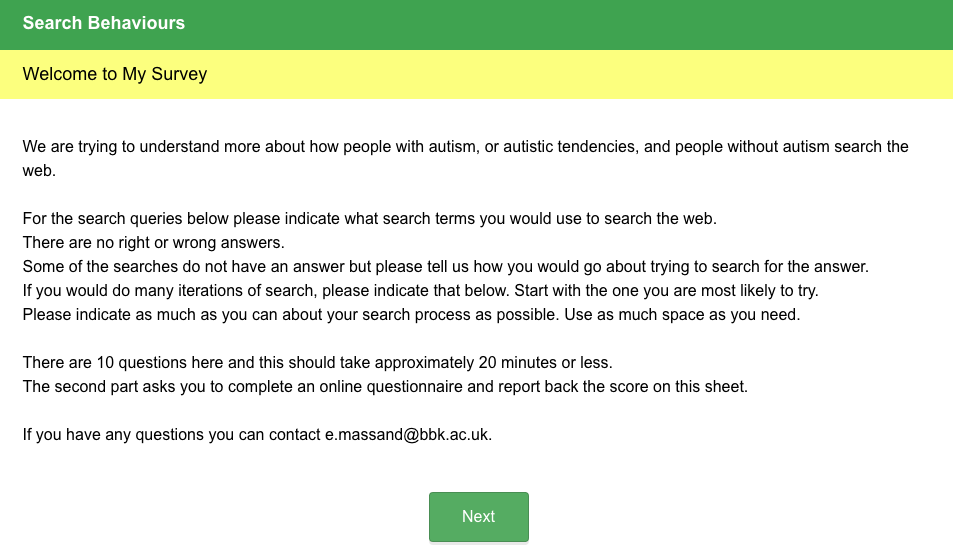
\includegraphics[scale=0.5]{survey1}\\
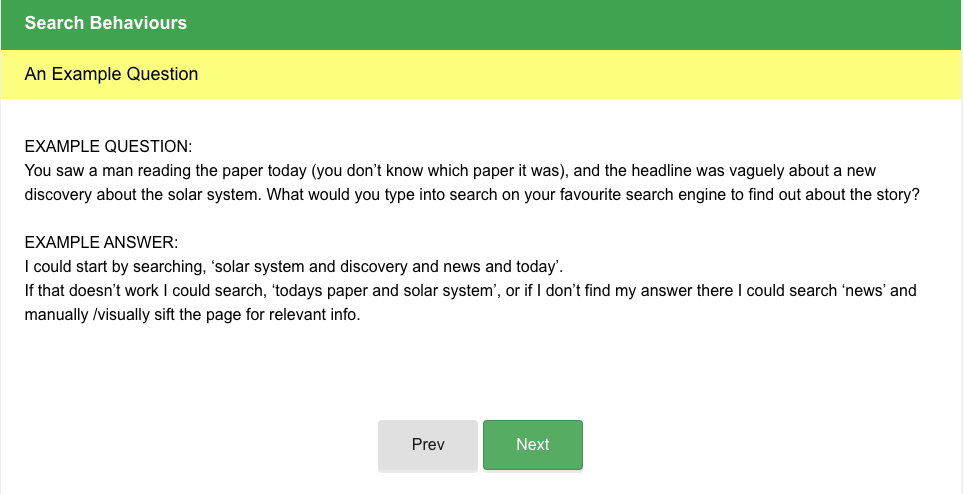
\includegraphics[scale=0.5]{survey2}\\
\end{center}
\end{figure}
\newpage
\begin{figure}[H]
\begin{center}
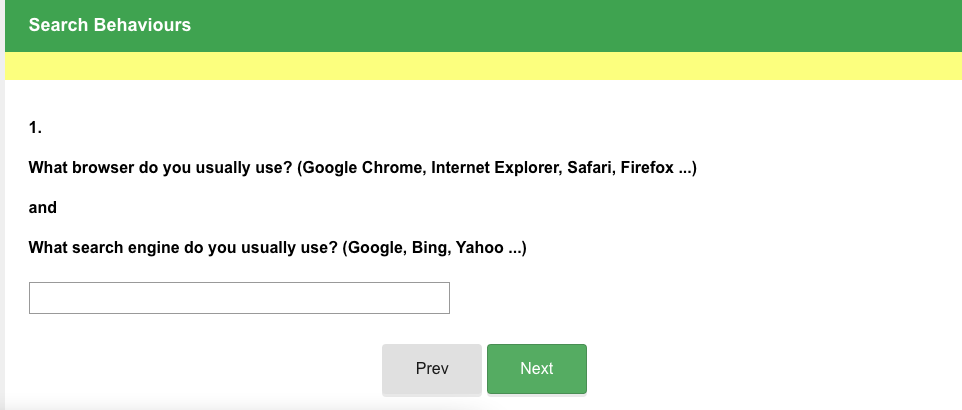
\includegraphics[scale=0.5]{survey3}\\
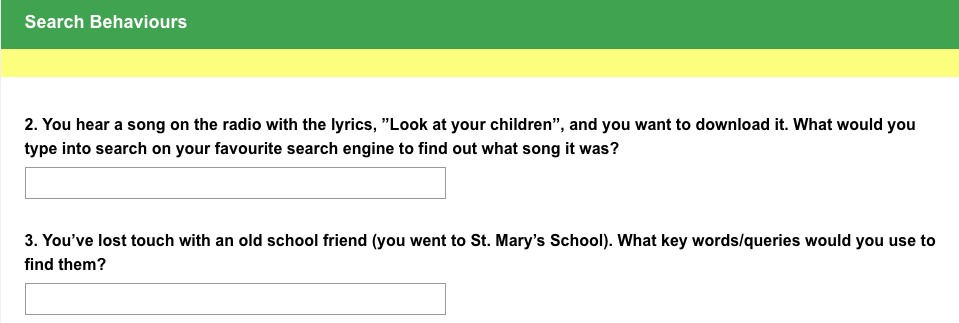
\includegraphics[scale=0.5]{survey4}\\
\end{center}
\end{figure}
\newpage
\begin{figure}[H]
\begin{center}
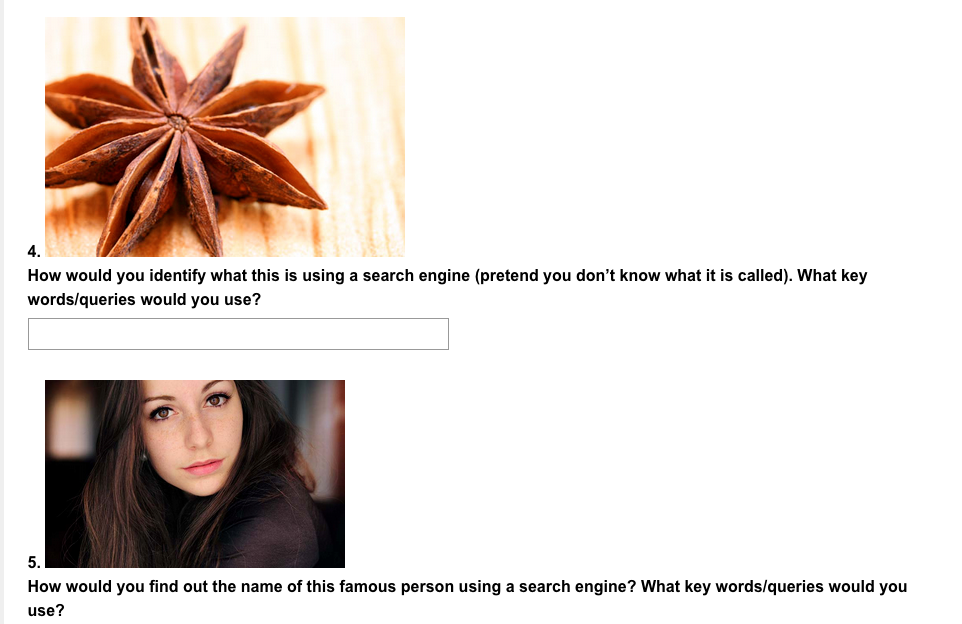
\includegraphics[scale=0.5]{survey5}\\
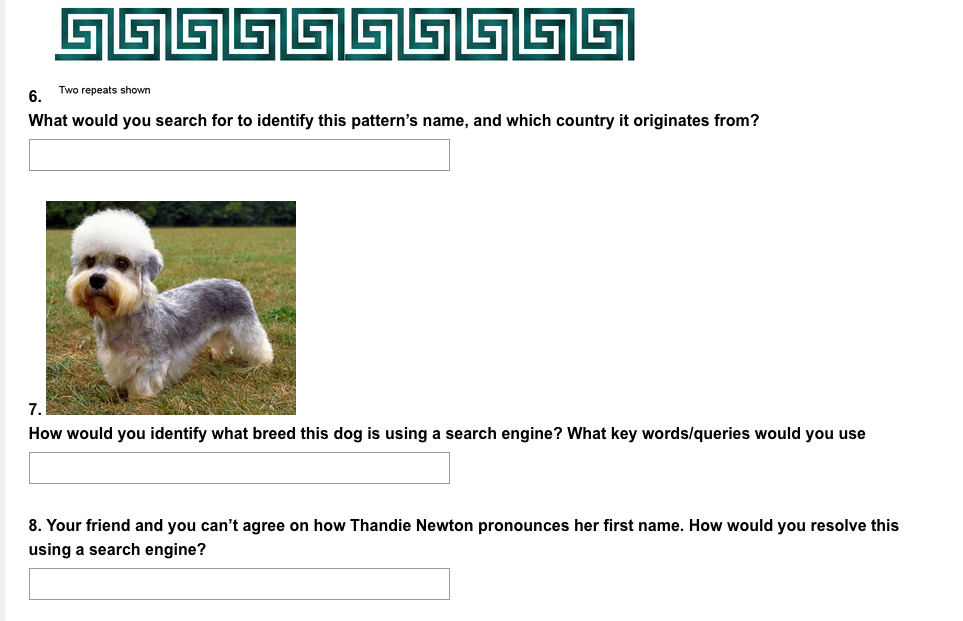
\includegraphics[scale=0.5]{survey6}\\
\end{center}
\end{figure}

\newpage
\begin{figure}[H]
\begin{center}
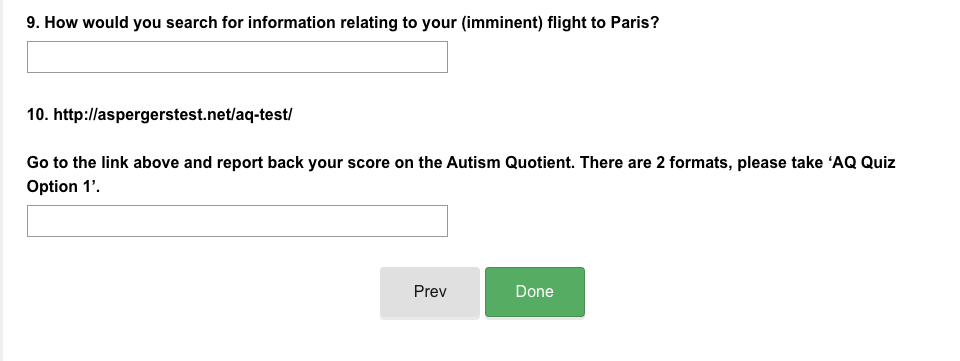
\includegraphics[scale=0.5]{survey7}\\
\caption{Search Query Survey on Surveymonkey.com \cite{surveymonkey}}
\end{center}
\end{figure}

\newpage
\subsection{Questions on the Autism Spectrum Quotient \cite{Baron Cohen et al}} \label{AQ}

Participants are asked to read each statement very carefully and rate how strongly they agree or disagree with the statement (Strongly Disagree, Slightly Disagree, Slightly Agree, or, Strongly Agree).  \\
\hspace{1cm}

I prefer to do things with others rather than on my own.\\
I prefer to do things the same way over and over again.\\
If I try to imagine something, I find it very easy to create a picture in my mind.\\
I frequently get so strongly absorbed in one thing that I lose sight of other things.\\
I often notice small sounds when others do not.\\
I usually notice car number plates or similar strings of information.\\
Other people frequently tell me that what I’ve said is impolite, even though I think it is polite.\\
When I'm reading a story, I can easily imagine what the characters might look like.\\
I am fascinated by dates.\\
In a social group, I can easily keep track of several different people’s conversations.\\
I find social situations easy.\\
I tend to notice details that others do not.\\
I would rather go to a library than a party.\\
I find making up stories easy.\\
I find myself drawn more strongly to people than to things.\\
I tend to have very strong interests which I get upset about if I can't pursue.\\
I enjoy social chit-chat.\\
When I talk, it isn't always easy for others to get a word in edgeways.\\
I am fascinated by numbers.\\
When I'm reading a story, I find it difficult to work out the characters' intentions.\\
I don't particularly enjoy reading fiction.\\
I find it hard to make new friends.\\
I notice patterns in things all the time.\\
I would rather go to the theatre than a museum.\\
It does not upset me if my daily routine is disturbed.\\
I frequently find that I don't know how to keep a conversation going.\\
I find it easy to read between the lines when someone is talking to me.\\
I usually concentrate more on the whole picture, rather than the small details.\\
I am not very good at remembering phone numbers.\\
I don’t usually notice small changes in a situation, or a person’s appearance.\\
I know how to tell if someone listening to me is getting bored.\\
I find it easy to do more than one thing at once.\\
When I talk on the phone, I'm not sure when it's my turn to speak.\\
I enjoy doing things spontaneously.\\
I am often the last to understand the point of a joke.\\
I find it easy to work out what someone is thinking or feeling just by looking at their face.\\
If there is an interruption, I can switch back to what I was doing very quickly. \\
I am good at social chit-chat.\\
People often tell me that I keep going on and on about the same thing.\\
When I was young, I used to enjoy playing games involving pretending with other children.\\
I like to collect information about categories of things (e.g. types of car, types of bird, types of train, types of plant, etc.).\\
I find it difficult to imagine what it would be like to be someone else.\\
I like to plan any activities I participate in carefully.\\
I enjoy social occasions.\\
I find it difficult to work out people's intentions.\\
New situations make me anxious.\\
I enjoy meeting new people.\\
I am a good diplomat.\\
I am not very good at remembering people's date of birth.\\
I find it very easy to play games with children that involve pretending.\\

\end{document} 